% Generated by book/tools/notebook_to_tex.py. Do not edit by hand.

\chapter[한국어 BERT 다중 클래스 분류 (Korean Multi-class Classification)]{한국어 BERT 다중 클래스 분류 (Korean Multi-class Classification)}

\label{ch:16}

\markboth{한국어 BERT 다중 클래스 분류 (Korean Multi-class Classification)}{한국어 BERT 다중 클래스 분류 (Korean Multi-class Classification)}

\chaptermeta{16_ko_multiclass/16_ko_multiclass.ipynb}{https://colab.research.google.com/github/yoon-gu/neuqes-101/blob/master/16_ko_multiclass/16_ko_multiclass.ipynb}{KLUE-YNAT 7분류로 한국어 BERT softmax 헤드를 K=7까지 확장}



\index{1KLUE YNAT@KLUE-YNAT}

\index{1Korean BERT@Korean BERT}

\index{1KLUE BERT@KLUE-BERT}

\index{1klue bert base@klue/bert-base}

\index{1multi class classification@multi-class classification}

\index{1CrossEntropyLoss@CrossEntropyLoss}

\index{1num labels 7@num\_labels=7}

\index{1confusion matrix@confusion\_matrix}

\index{1top 1 probability@top-1 probability}

\index{1macro F1@macro F1}

\index{0한국어 BERT@한국어 BERT}

\index{0한국어 다중 클래스 분류@한국어 다중 클래스 분류}

\index{0뉴스 분류@뉴스 분류}

\index{0혼동 행렬@혼동 행렬}

\index{0최상위 확률@최상위 확률}

\index{0매크로 F1@매크로 F1}

\index{1load dataset klue ynat@load\_dataset("klue", "ynat")}

\index{1problem type single label classification@problem\_type="single\_label\_classification"}

\index{1roc auc score@roc\_auc\_score}

\index{1multi class ovr@multi\_class="ovr"}

\index{1seaborn heatmap@seaborn.heatmap}

\index{07분류@7분류}

\index{0행 정규화 혼동 행렬@행 정규화 혼동 행렬}

\index{0캘리브레이션@캘리브레이션}



\section{변화추적표}

\begin{booktable}{16장 변화추적표}{tab:ch16-01}
\begin{adjustbox}{max width=\textwidth}
\begin{tabular}{@{}lllllll@{}}
\toprule
Ch & 모델 & 토크나이저 & 데이터 & Output Head & Activation & Loss \\
\midrule

12 & DistilBERT & WordPiece (영어) & Yelp 5클래스 & \inlinecode{Linear(H,\ 5)} & softmax & \inlinecode{CrossEntropyLoss} \\
15 & klue/bert-base & WordPiece (한국어) & NSMC binary & \inlinecode{Linear(H,\ 2)} & softmax & \inlinecode{CrossEntropyLoss} \\
\textbf{16 \(\leftarrow\) 여기} & klue/bert-base & 같음 & \textbf{KLUE-YNAT (뉴스 7분류)} & \textbf{\inlinecode{Linear(H,\ 7)}} & softmax & \inlinecode{CrossEntropyLoss} \\
17 (다음) & klue/bert-base & 같음 & KLUE-YNAT 합성 multi-label & \inlinecode{Linear(H,\ 7)} & sigmoid (per-label) & \inlinecode{BCEWithLogitsLoss} (per-label) \\
\bottomrule
\end{tabular}
\end{adjustbox}
\end{booktable}

전체 장 표는 \href{https://github.com/yoon-gu/neuqes-101\#챕터별-변화추적표}{루트 README.md}를 참고하세요.



\section{변경점: \ref{ch:15}장 대비}

\begin{booktable}{16장 변경점 요약}{tab:ch16-02}
\begin{adjustbox}{max width=\textwidth}
\begin{tabular}{@{}lll@{}}
\toprule
축 & \ref{ch:15}장 (한국어 binary) & \ref{ch:16}장 (한국어 multi-class) \\
\midrule

\textbf{Task} & 이진 분류 (K=2) & \textbf{7-클래스 분류 (K=7)} \(\leftarrow\) \emph{유일한 변화} \\
\inlinecode{num\_labels} & 2 & \textbf{7} \\
데이터 & NSMC (영화 리뷰) & \textbf{KLUE-YNAT (뉴스 헤드라인)} \\
라벨 형식 & int 0/1 & \textbf{int 0-6} \\
평가 metric & binary precision/recall/F1 + AUC & \textbf{accuracy + macro precision/recall/F1 + multi-class AUC (OvR)} \\
모델 / 토크나이저 / problem\_type / Activation / Loss / hyperparams & (모두 동일) & (모두 동일) \\
\bottomrule
\end{tabular}
\end{adjustbox}
\end{booktable}

\begin{quote}
\textbf{변경점 한 가지 원칙} --- Phase 2 안에선 \emph{task 차원} (K=2 \(\to\) K=7) 만 바뀝니다. 한국어 셋업·hyperparams 는 \ref{ch:15}장과 \emph{완전히 같음}. 새 장의 학습 부담은 \emph{7클래스 평가 metric 의 해석} 에만 집중.
\end{quote}

\subsection{\texorpdfstring{한국어 환경에서도 multi-class 일반화는 \emph{그대로} 작동}{한국어 환경에서도 multi-class 일반화는 그대로 작동}}

\ref{ch:11}장 \(\to\) \ref{ch:12}장 (영어 binary \(\to\) multi-class) 에서 \inlinecode{num\_labels} 를 2 \(\to\) 5 로만 바꿔도 모든 셋업이 그대로 동작했습니다. \ref{ch:15}장 \(\to\) \ref{ch:16}장도 정확히 같은 패턴 --- \emph{softmax+CE 의 진짜 강점}: K 가 무엇이든 같은 식으로 일반화됩니다.



\section{\texorpdfstring{손실 노트 --- \inlinecode{CrossEntropyLoss} 가 K=7 에서 보이는 모습}{손실 노트 --- CrossEntropyLoss 가 K=7 에서 보이는 모습}}

수식은 \ref{ch:12}장과 동일:

\begin{equation}
\label{eq:ch16-01}
L = -\frac{1}{N}\sum_{i=1}^{N}\log \hat p_{i, y_i}
\end{equation}

식~\eqref{eq:ch16-01}은 이 절에서 사용하는 핵심 관계를 정리한 것입니다.

K=7 의 random baseline loss = \(\log 7 = 1.946\). 학습 첫 step 에서 loss 가 \textasciitilde1.9 정도 보이면 모델이 \emph{균등 추측 단계} --- 이후 loss 가 떨어지는 곡선이 학습이 \emph{실제로 진행되는지} 진단 신호.

\textbf{숫자로 감 잡기 (K=7, 정답 = 클래스 5)}:

\begin{booktable}{16장 손실 수치 예시}{tab:ch16-03}
\begin{adjustbox}{max width=\textwidth}
\begin{tabular}{@{}lll@{}}
\toprule
logits & softmax \(\to\) \(\hat p_5\) & 손실 \\
\midrule

모두 0 (균등) & \(1/7 \approx 0.143\) & \textbf{1.946} \(\leftarrow\) random \\
정답 클래스만 +2 & \(\approx 0.552\) & 0.594 \\
정답 클래스만 +5 & \(\approx 0.961\) & 0.040 \\
다른 클래스 하나만 +5 (정답 0) & \(\approx 0.006\) & \textbf{5.040} \(\leftarrow\) 자신 있게 틀림 \\
\bottomrule
\end{tabular}
\end{adjustbox}
\end{booktable}

\textbf{클래스 균형 영향} --- KLUE-YNAT 의 클래스 분포는 \emph{완벽 균형이 아닙니다} (스포츠/세계가 정치/IT보다 많음). class\_weight 없이 학습하면 \emph{다수 클래스} 에 편향될 가능성. 평가 단계에서 \emph{macro F1} 을 같이 봐야 소수 클래스 정확도가 묻히지 않음.



\section{토크나이저 노트}

\ref{ch:15}장과 \emph{완전히 동일} --- \inlinecode{klue/bert-base} 한국어 WordPiece. 토크나이저는 K 변화에 무관 (라벨 처리는 모델 측 일).

\begin{quote}
\textbf{Phase 2 안에서는 토크나이저 고정} --- \ref{ch:15}·\ref{ch:16}장·17·18 모두 같은 한국어 WordPiece. Phase 3 (\ref{ch:19}--\ref{ch:23}장) 에서 비로소 \emph{직접 학습한 워드레벨 토크나이저} 가 등장.
\end{quote}

\subsection{헤드라인 토큰화 예시}

NSMC 영화 리뷰는 보통 \emph{짧은 한 줄} (약 20 토큰), KLUE-YNAT 뉴스 헤드라인도 비슷하게 짧아 \emph{평균 약 16 토큰 (최대 27)}. 같은 한국어지만 \emph{문체가 다른} 두 도메인 --- 도메인 적응이 어떻게 이뤄지는지 확인할 좋은 비교.



\textbf{baseline VRAM}:



\Needspace{5\baselineskip}
\begin{lstlisting}
!nvidia-smi
\end{lstlisting}

\begin{codeRead}
\textbf{1행}의 \inlinecode{!nvidia-smi}에서는 앞 단계에서 만든 값을 바탕으로 다음 계산을 수행합니다.
\end{codeRead}



\section{데이터 준비}

\textbf{KLUE} = Korean Language Understanding Evaluation 벤치마크. \textbf{YNAT} = Yonhap News Agency Topic. 연합뉴스 헤드라인 한 줄 + 7카테고리 라벨.

\begin{booktable}{16장 데이터 준비 표}{tab:ch16-04}
\begin{adjustbox}{max width=\textwidth}
\begin{tabular}{@{}ll@{}}
\toprule
라벨 & 카테고리 \\
\midrule

0 & IT과학 \\
1 & 경제 \\
2 & 사회 \\
3 & 생활문화 \\
4 & 세계 \\
5 & 스포츠 \\
6 & 정치 \\
\bottomrule
\end{tabular}
\end{adjustbox}
\end{booktable}

\inlinecode{datasets.load\_dataset("klue/klue",\ "ynat")} 로 정상 로드 (parquet 기반).



\Needspace{11\baselineskip}
\begin{lstlisting}
SEED = 42
train_full = ds["train"].shuffle(seed=SEED).select(range(5000))
eval_full  = ds["validation"].shuffle(seed=SEED).select(range(1000))

train_full = train_full.rename_column("title", "text")
eval_full  = eval_full.rename_column("title", "text")

print(f"sampled train: {len(train_full)}")
print(f"sampled eval:  {len(eval_full)}")

tokenizer = AutoTokenizer.from_pretrained("klue/bert-base")
sample_lens = [len(tokenizer.encode(t)) for t in train_full["text"][:200]]
print(
    f"\nToken length (sample 200): mean={np.mean(sample_lens):.1f}, median={np.median(sample_lens):.0f}, max="
    f"{max(sample_lens)}"
)
\end{lstlisting}



\section{토큰화 --- \ref{ch:15}장 패턴 그대로}

라벨 형식만 binary int \(\to\) 0-6 int. 한 줄 차이.



\Needspace{11\baselineskip}
\begin{lstlisting}
def tokenize_fn(batch):
    out = tokenizer(
        batch["text"],
        truncation=True,
        max_length=128,
    )
    out["labels"] = [int(l) for l in batch["label"]]
    return out

train_tok = train_full.map(tokenize_fn, batched=True).remove_columns(
    [c for c in train_full.column_names if c not in ("input_ids", "attention_mask", "token_type_ids", "labels")]
)
eval_tok  = eval_full.map(tokenize_fn,  batched=True).remove_columns(
    [c for c in eval_full.column_names if c not in ("input_ids", "attention_mask", "token_type_ids", "labels")]
)

\end{lstlisting}

\noindent\emph{앞 블록은 텍스트를 모델 입력 텐서로 바꾸는 단계입니다. 이어지는 블록에서는 앞에서 만든 중간 값을 다음 계산으로 넘기는 단계로 넘어갑니다.}

\Needspace{7\baselineskip}
\begin{lstlisting}[firstnumber=17]
print(train_tok)
print(
    f"\nFirst sample label: "
    f"{train_tok[0]['labels']}  (int 0-6)"
)
\end{lstlisting}

\noindent\textbf{출력.}
\begin{bookoutputbox}
Dataset({
    features: ['input_ids', 'token_type_ids', 'attention_mask', 'labels'],
    num_rows: 5000
})

First sample label: 3  (int 0-6)
\end{bookoutputbox}
\par\vspace{0.9em}



\section{\texorpdfstring{모델 로드}{모델 로드}}

\ref{ch:15}장 셋업에서 K=2 \(\to\) K=7 한 줄 변화.



\Needspace{11\baselineskip}
\begin{lstlisting}
model = AutoModelForSequenceClassification.from_pretrained(
    "klue/bert-base",
    num_labels=len(LABEL_NAMES),
    problem_type="single_label_classification",
    id2label={i: name for i, name in enumerate(LABEL_NAMES_EN)},
    label2id={name: i for i, name in enumerate(LABEL_NAMES_EN)},
)

def param_summary(m):
    total     = sum(p.numel() for p in m.parameters())
    trainable = sum(p.numel() for p in m.parameters() if p.requires_grad)
    return total, trainable

\end{lstlisting}

\noindent\emph{앞뒤 블록은 모두 앞에서 만든 중간 값을 다음 계산으로 넘기는 단계입니다. 길이를 나누어 같은 흐름을 단계별로 확인합니다.}

\Needspace{11\baselineskip}
\begin{lstlisting}[firstnumber=14]
total, trainable = param_summary(model)
print(
    f"Parameters:           {total:>13,}  ("
    f"{total/1e6:.1f} M)"
)
print(
    f"Trainable parameters: {trainable:>13,}  ("
    f"{trainable/total:.1%})"
)
print(f"Classifier:           {model.classifier}")
print(f"id2label:             {model.config.id2label}")
\end{lstlisting}

\noindent\textbf{출력.}
\begin{bookoutputbox}
Key                                        | Status     | 
-------------------------------------------+------------+-
classifier.bias                            | MISSING    | 
classifier.weight                          | MISSING    | 

- MISSING: those params were newly initialized because missing from the che...
Parameters:             110,622,727  (110.6 M)
Trainable parameters:   110,622,727  (100.0%)
Classifier:           Linear(in_features=768, out_features=7, bias=True)
id2label: {0: 'IT/Science', 1: 'Economy', 2: 'Society', 3: 'Life&Culture',...
\end{bookoutputbox}
\par\vspace{0.9em}



\textbf{\ref{ch:15}장과의 파라미터 수 비교} --- 7클래스로 늘어났는데도 모델은 \emph{거의 안 무거워짐}:

\begin{booktable}{16장 모델 로드 표}{tab:ch16-05}
\begin{adjustbox}{max width=\textwidth}
\begin{tabular}{@{}lll@{}}
\toprule
부분 & \ref{ch:15}장 (K=2) & \ref{ch:16}장 (K=7) \\
\midrule

BERT body (12 layer) & 110,617,344 & 110,617,344 \\
classifier \inlinecode{Linear(768,\ K)} & 1,538 & \textbf{5,383} \\
합계 & 110,618,882 & \textbf{110,622,727} \\
\bottomrule
\end{tabular}
\end{adjustbox}
\end{booktable}

분류 헤드만 K 에 비례해 늘어나지만 BERT body 가 \textasciitilde110M 이라 K 가 5 늘어도 전체 차이는 0.003\%. \textbf{K 가 늘어났다고 학습이 \emph{훨씬} 무거워지지는 않는다} --- multi-class BERT 의 매력.



\Needspace{5\baselineskip}
\begin{lstlisting}
!nvidia-smi
\end{lstlisting}



\section{학습}

\inlinecode{compute\_metrics} 만 multi-class 용으로 (\ref{ch:12}장의 패턴 그대로).



\Needspace{11\baselineskip}
\begin{lstlisting}
def compute_metrics(eval_pred):
    logits, labels = eval_pred

    exp = np.exp(logits - logits.max(axis=1, keepdims=True))
    probs_full = exp / exp.sum(axis=1, keepdims=True)
    preds = probs_full.argmax(axis=1)

    p, r, f1, _ = precision_recall_fscore_support(
        labels,
        preds,
        average="macro",
        zero_division=0,
    )
    out = {
        "accuracy":        float(accuracy_score(labels, preds)),
        "macro_precision": float(p),
\end{lstlisting}

\noindent\emph{앞 블록은 예측 결과를 지표와 표로 요약하는 단계입니다. 이어지는 블록에서는 앞에서 만든 중간 값을 다음 계산으로 넘기는 단계로 넘어갑니다.}

\Needspace{11\baselineskip}
\begin{lstlisting}[firstnumber=17]
        "macro_recall":    float(r),
        "macro_f1":        float(f1),
    }
    # multi-class AUC: One-vs-Rest
    try:
        out["auc_ovr"] = float(roc_auc_score(labels, probs_full, multi_class="ovr"))
    except ValueError:
        out["auc_ovr"] = float("nan")
    return out
\end{lstlisting}



\Needspace{5\baselineskip}
\begin{lstlisting}
!nvidia-smi
\end{lstlisting}



\section{평가}

\ref{ch:12}장의 평가 패턴을 한국어 환경에서 재현. 7클래스라 혼동 행렬이 7\(\times\)7 --- \emph{어떤 카테고리가 어떤 카테고리와 혼동하는지} 보는 데 핵심.



\Needspace{11\baselineskip}
\begin{lstlisting}
preds_output = trainer.predict(eval_tok)
logits = preds_output.predictions
labels = preds_output.label_ids.astype(int)

exp = np.exp(logits - logits.max(axis=1, keepdims=True))
probs_full = exp / exp.sum(axis=1, keepdims=True)
preds = probs_full.argmax(axis=1)

top1_prob = probs_full.max(axis=1)
correct = (preds == labels)

\end{lstlisting}

\noindent\emph{앞 블록은 학습 설정을 만들고 학습 루프를 실행하는 단계입니다. 이어지는 블록에서는 모델 출력을 확률이나 예측값으로 바꾸는 단계로 넘어갑니다.}

\Needspace{11\baselineskip}
\begin{lstlisting}[firstnumber=12]
print(f"logits shape:    {logits.shape}")
print(
    f"top-1 prob range: [{top1_prob.min():.4f}, "
    f"{top1_prob.max():.4f}]"
)
print(
    f"top-1 prob mean: correct={top1_prob[correct].mean():.4f}, wrong="
    f"{top1_prob[~correct].mean():.4f}"
)
\end{lstlisting}

\begin{codeRead}
\textbf{1행}의 \inlinecode{preds\_output = ...}에서는 학습된 모델로 최종 예측값을 만듭니다. \textbf{2행}의 \inlinecode{logits = ...}에서는 이후 분석에서 사용할 값을 준비합니다. \textbf{3행}의 \inlinecode{labels = ...}에서는 이후 분석에서 사용할 값을 준비합니다.
\end{codeRead}



\Needspace{7\baselineskip}
\begin{lstlisting}
print(classification_report(
    labels, preds,
    target_names=LABEL_NAMES_EN,
    digits=4, zero_division=0,
))
\end{lstlisting}

\noindent\textbf{출력.}
\begin{bookoutputbox}
precision    recall  f1-score   support

  IT/Science     0.7857    0.9483    0.8594        58
     Economy     0.8210    0.8471    0.8339       157
     Society     0.8830    0.8300    0.8557       400
Life&Culture     0.8129    0.8630    0.8372       146
       World     0.9053    0.8866    0.8958        97
      Sports     0.9459    0.9459    0.9459        74
    Politics     0.7941    0.7941    0.7941        68

    accuracy                         0.8560      1000
   macro avg     0.8497    0.8736    0.8603      1000
weighted avg     0.8582    0.8560    0.8562      1000
\end{bookoutputbox}
\par\vspace{0.9em}



\subsection{혼동 행렬 --- 어디서 혼동하는가}

행은 정답 카테고리, 열은 예측. 색은 \emph{행 정규화 (recall)}, 숫자는 \emph{원본 카운트}. 대각선이 진할수록 그 카테고리 재현율이 좋음.



\compactCodeOmitted{예측 결과를 지표와 표로 요약하는 단계}

\begin{bookfigurelabel}[H]{KLUE-YNAT 7분류 혼동 행렬}{fig:ch16-confusion-matrix}
\centering
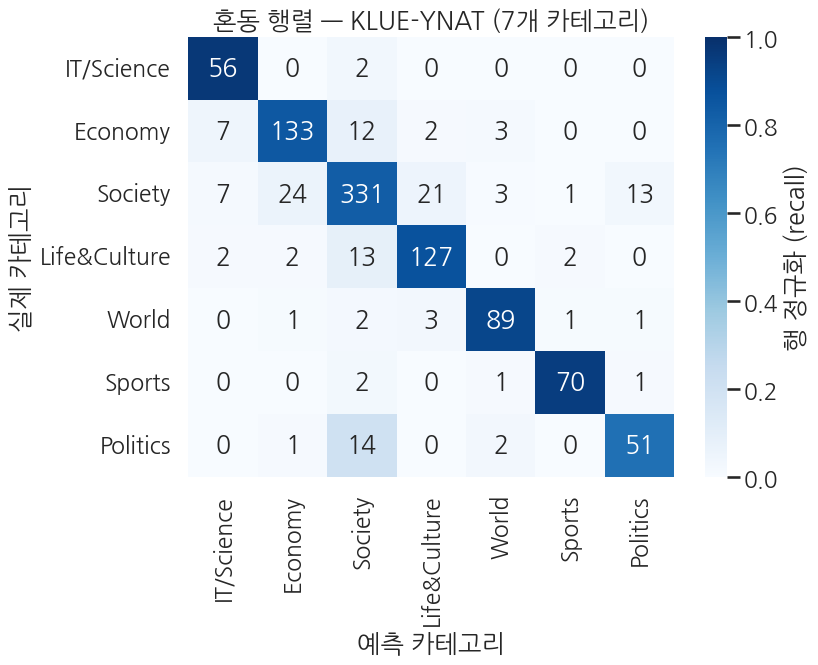
\includegraphics[width=0.86\linewidth]{assets/figures/ch16_confusion_matrix.png}
\end{bookfigurelabel}

\textbf{그림 읽기} --- 그림~\ref{fig:ch16-confusion-matrix}에서 다음 내용을 확인합니다: KLUE-YNAT 7분류 혼동 행렬. 실행된 노트북에서 저장된 최신 plot 출력이므로, 코드에서 계산한 값이 어떤 평가 지점으로 이어지는지 바로 확인할 수 있습니다.



\textbf{해석 가이드}

\begin{itemize}
\tightlist
\item
  \textbf{대각선 셀} = 그 카테고리의 재현율. 모든 셀이 0.85+ 면 잘 학습된 것.
\item
  \textbf{오답 패턴}:

  \begin{itemize}
  \tightlist
  \item
    정치 \(\leftrightarrow\) 경제: 둘 다 정책·법안·국제 이슈 다뤄 \emph{경계가 모호} --- 자연스러운 혼동
  \item
    생활문화 \(\leftrightarrow\) 사회: 사회 이슈 vs 일상·문화 보도 --- 헤드라인 한 줄로는 사람도 혼동하는 경계
  \item
    IT과학 \(\leftrightarrow\) 경제: 기업·산업 뉴스가 양쪽에 걸침 (예: “삼성전자 4분기 실적 발표”)
  \end{itemize}
\item
  \textbf{먼 클래스 혼동} (스포츠 \(\leftrightarrow\) 정치 등) 이 자주 보이면 라벨 노이즈나 학습 부족 신호.
\end{itemize}



\subsection{최상위 확률 분포}

K=7 에선 \emph{어느 한 클래스에 압도적 자신} 있는 경우 vs \emph{2-3 후보 사이에서 갈등} 하는 경우가 나뉩니다. correct/wrong 으로 갈라 그려 calibration 확인.



\compactCodeOmitted{숫자 결과를 그림으로 확인하는 단계}

\begin{bookfigurelabel}[H]{정답 여부에 따른 KLUE-YNAT 최상위 확률 분포}{fig:ch16-top1-probability}
\centering
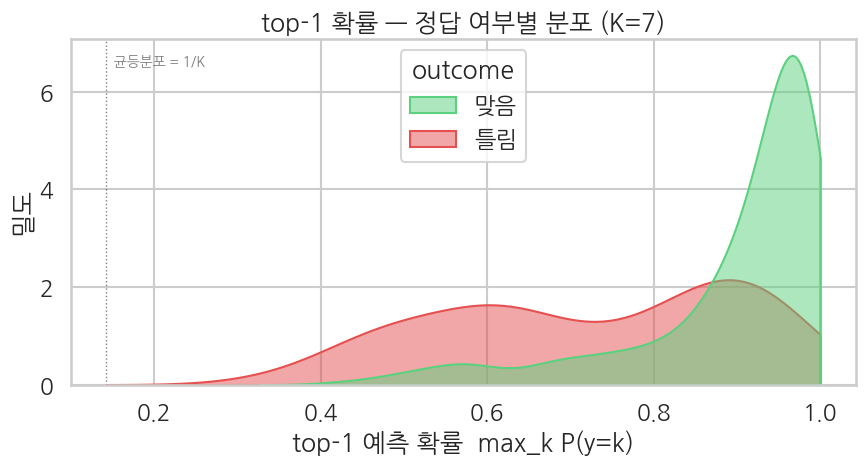
\includegraphics[width=0.88\linewidth]{assets/figures/ch16_top1_probability.png}
\end{bookfigurelabel}

\textbf{그림 읽기} --- 그림~\ref{fig:ch16-top1-probability}에서 다음 내용을 확인합니다: 정답 여부에 따른 KLUE-YNAT 최상위 확률 분포. 실행된 노트북에서 저장된 최신 plot 출력이므로, 코드에서 계산한 값이 어떤 평가 지점으로 이어지는지 바로 확인할 수 있습니다.



\textbf{해석}

\begin{itemize}
\tightlist
\item
  잘 학습된 모델은 \emph{correct} 곡선이 1.0 가까이 몰림. \emph{wrong} 은 더 낮은 영역 (0.4-0.7) 에 분산.
\item
  correct/wrong 둘 다 1.0 근처에 압축돼 있으면 \emph{over-confident} --- 틀린 답에도 자신만만한 위험 신호. K 가 클수록 (7클래스) 이런 경향이 더 잘 드러남.
\item
  \emph{random baseline} 인 1/K = 0.143 근처 봉우리가 보이면 모델이 \emph{판단 자체를 못 하는} 샘플 --- 학습 데이터 부족 또는 헤드라인이 너무 짧은 경우.
\end{itemize}



\subsection{샘플 단위 해석}

가장 자신있는 샘플 / 망설이는 샘플 / 자신있게 틀린 샘플 세 종류를 골라 직접 읽어 봅니다. 헤드라인 한 줄 만으로 모델이 어떤 카테고리 신호를 잡는지 감각.



\Needspace{11\baselineskip}
\begin{lstlisting}
texts = list(eval_full["text"])

idx_top    = int(np.argmax(top1_prob))
idx_unc    = int(np.argmin(np.abs(top1_prob - 1/len(LABEL_NAMES) * 2)))
wrong_mask = ~correct
idx_wrong  = int(np.argmax(top1_prob * wrong_mask)) if wrong_mask.any() else -1

samples = [
    ("most confident overall", idx_top),
    ("most uncertain (~2/K)", idx_unc),
    ("most confident WRONG",   idx_wrong),
]

\end{lstlisting}

\noindent\emph{앞 블록은 앞에서 만든 중간 값을 다음 계산으로 넘기는 단계입니다. 이어지는 블록에서는 모델 출력을 확률이나 예측값으로 바꾸는 단계로 넘어갑니다.}

\Needspace{11\baselineskip}
\begin{lstlisting}[firstnumber=14]
for label_str, idx in samples:
    if idx < 0:
        continue
    print("=" * 78)
    print(f"sample #{idx}  ({label_str})")
    print("=" * 78)
    print(f"text:        {texts[idx]}")
    print(
        f"true label:  {labels[idx]}  ("
        f"{LABEL_NAMES[labels[idx]]})"
    )
    print(
        f"prediction:  {preds[idx]}  ({LABEL_NAMES[preds[idx]]})  match: "
        f"{'OK' if correct[idx] else 'X'}"
    )
    print(f"top-1 prob:  {top1_prob[idx]:.4f}")
\end{lstlisting}

\noindent\emph{앞 블록은 모델 출력을 확률이나 예측값으로 바꾸는 단계입니다. 이어지는 블록에서는 앞에서 만든 중간 값을 다음 계산으로 넘기는 단계로 넘어갑니다.}

\Needspace{10\baselineskip}
\begin{lstlisting}[firstnumber=30]
    top3 = np.argsort(probs_full[idx])[::-1][:3]
    print(f"top-3 distribution:")
    for k in top3:
        print(
            f"  {LABEL_NAMES[k]:>8}: "
            f"{probs_full[idx, k]:.4f}"
        )
    print()
\end{lstlisting}



\textbf{관찰 포인트}

\begin{itemize}
\tightlist
\item
  \emph{가장 자신있는} 샘플은 보통 카테고리 \emph{시그널 단어} 가 명확 (예: “주가” \(\to\) 경제, “월드컵” \(\to\) 스포츠).
\item
  \emph{망설이는 샘플} 의 top-3 분포를 보면 모델이 \emph{어느 카테고리 사이에서 갈팡질팡} 하는지 보임. 정치/경제/사회 셋이 비슷한 확률이면 헤드라인 자체가 다중 카테고리에 걸침.
\item
  \emph{자신있게 틀린} 샘플은 보통 \emph{반어}, \emph{비유}, \emph{카테고리 간 경계 사례} --- 학습 데이터에 비슷한 패턴이 없었거나 라벨 자체가 모호. 이걸 보면 “모델이 \emph{바보} 라서 틀린 게 아니라 \emph{데이터가 어렵다} ” 는 감각 잡힘.
\end{itemize}



\section{이 장에 등장한 라이브러리·함수}

\begin{booktable}{16장 새로 등장한 라이브러리}{tab:ch16-06}
\begin{adjustbox}{max width=\textwidth}
\begin{tabular}{@{}lll@{}}
\toprule
이름 & 한 줄 설명 & 다음 장에서 \\
\midrule

\inlinecode{load\_dataset("klue/klue",\ "ynat")} & KLUE 벤치마크 YNAT (한국어 뉴스 7분류) & \ref{ch:17}장에서 같은 데이터로 multi-label 합성 \\
\texttt{ds{[}“train”{]}.features{[}“label”{]}.names} & datasets.ClassLabel 의 사람-읽는 이름 & id2label 자동 매핑에 사용 \\
\inlinecode{seaborn.heatmap(...,\ xticklabels=한국어)} & 혼동 행렬 한국어 라벨 표시 & \ref{ch:17}장도 사용 \\
\inlinecode{sklearn.metrics.precision\_recall\_fscore\_support(...,\ average="macro")} & 클래스별 평균 metric (불균형에 강함) & 분류 장마다 \\
\inlinecode{roc\_auc\_score(...,\ multi\_class="ovr")} & multi-class AUC (One-vs-Rest) & \ref{ch:17}장 multi-label 평가 \\
\bottomrule
\end{tabular}
\end{adjustbox}
\end{booktable}



\section{체크포인트 질문}

\begin{enumerate}
\def\labelenumi{\arabic{enumi}.}
\tightlist
\item
  K=7 학습 첫 step 의 loss 가 약 1.95 정도라면 모델이 무엇을 학습한 상태인가요?
\item
  macro F1 이 weighted F1 보다 \emph{훨씬} 낮으면 무엇을 의심해야 하나요?
\item
  혼동 행렬에서 \emph{정치 \(\leftrightarrow\) 경제} 혼동이 많은데 \emph{스포츠 \(\leftrightarrow\) 정치} 혼동은 거의 없는 이유는?
\item
  같은 klue/bert-base 가 NSMC binary (\ref{ch:15}장) 와 KLUE-YNAT 7분류 (\ref{ch:16}장) 에서 \emph{분류 헤드만} 다른데, 왜 두 task 모두 잘 동작하나요?
\end{enumerate}



\section{FAQ}

\begin{faqBox}{Q1. (실무) 한국어 multi-class 데이터셋이 KLUE-YNAT 외에 어떤 게 있나요?}

\begin{booktable}{16장 FAQ 표}{tab:ch16-07}
\begin{adjustbox}{max width=\textwidth}
\begin{tabular}{@{}llll@{}}
\toprule
데이터셋 & 도메인 & 클래스 수 & 크기 \\
\midrule

\textbf{KLUE-YNAT} (이 장) & 뉴스 헤드라인 & 7 & 45K train \\
AI Hub 뉴스 분류 & 뉴스 본문 & 50+ & 100K+ (가입 필요) \\
모두의 말뭉치 신문 코퍼스 & 신문 기사 & 다양 & 매우 큼 (라이선스 확인 필요) \\
Naver shopping 카테고리 분류 & 상품 설명 & 100+ & 1M+ (실무에선 흔히 다룸) \\
\bottomrule
\end{tabular}
\end{adjustbox}
\end{booktable}

KLUE 벤치마크의 TC(Topic Classification) task 가 곧 YNAT 입니다 --- 별도 데이터셋이 아닙니다. KLUE-YNAT 가 \emph{입문에 편한 이유} --- datasets.load\_dataset 한 줄, 깔끔한 라벨, 균형 분포에 가까움, 헤드라인 한 줄이라 max\_length 짧음.

\end{faqBox}

\begin{faqBox}{Q2. (이론) 혼동 행렬에서 \emph{대칭} 인 혼동과 \emph{비대칭} 인 혼동은 무슨 차이인가요?}

\begin{itemize}
\tightlist
\item
  \textbf{대칭 혼동} (예: 정치\(\leftrightarrow\)경제 양방향 비슷): 두 카테고리 \emph{경계가 모호} 하다는 신호. 헤드라인 한 줄로는 \emph{사람도 혼동하는} 데이터.
\item
  \textbf{비대칭 혼동} (예: 정치 \(\to\) 경제 는 흔한데 경제 \(\to\) 정치 는 드뭄): 모델이 \emph{한쪽으로 편향} 됨. 가능한 원인:

  \begin{itemize}
  \tightlist
  \item
    학습 데이터 \emph{클래스 불균형} (한쪽이 많아 그쪽으로 답을 미는 경향)
  \item
    \emph{시그널 단어} 가 한쪽에 더 강하게 학습됨 (예: “정부”, “정책” 이 정치 카테고리에 너무 강하게 매핑)
  \end{itemize}
\end{itemize}

비대칭 혼동이 보이면 \inlinecode{class\_weight} 적용 또는 \emph{under-represented 클래스 oversampling} 으로 처치.

\end{faqBox}




\begin{faqBox}{Q6. (실무) 클래스 수가 50, 100 으로 늘면 같은 코드가 동작하나요?}

코드는 그대로 동작합니다 (\inlinecode{num\_labels=100} 만 바꾸면 됨). 하지만 \emph{학습 동역학} 이 달라집니다:

\begin{booktable}{16장 FAQ 표}{tab:ch16-08}
\begin{adjustbox}{max width=\textwidth}
\begin{tabular}{@{}lll@{}}
\toprule
K & random baseline loss & 학습 도전 \\
\midrule

7 (이 장) & \(\log 7 = 1.95\) & 무난 \\
50 & \(\log 50 = 3.91\) & 학습 데이터가 \emph{클래스당 충분} 해야 \\
100 & \(\log 100 = 4.60\) & 클래스 불균형이 심하면 자주 collapse \\
1000 & \(\log 1000 = 6.91\) & hierarchical softmax 등 특수 기법 고려 \\
\bottomrule
\end{tabular}
\end{adjustbox}
\end{booktable}

K 가 50+ 가 되면 \emph{클래스당 학습 샘플} 이 핵심 --- 클래스당 100 개 미만이면 BERT 정확도 떨어짐. KLUE-YNAT 는 클래스당 5K-8K 라 \emph{풍족한} 셋업.
\end{faqBox}



\compactFAQMore{3}

\section{오류 실험 (선택)}

다음 코드를 돌려보면 어떤 결과가 나올까요?

\Needspace{6\baselineskip}
\begin{lstlisting}
model_wrong = AutoModelForSequenceClassification.from_pretrained(
    "klue/bert-base",
    num_labels=2,
)
\end{lstlisting}

힌트: 학습 시 \inlinecode{CrossEntropyLoss(logits.shape=(B,\ 2),\ targets\ in\ 0-6)} 가 호출되는데 target 값이 logits 의 클래스 차원 범위를 \emph{벗어남} \(\to\) IndexError 또는 \emph{runtime cuda assert}. 모델 헤드가 라벨 범위와 \emph{일치해야} 한다는 단순하지만 흔한 실수.



\begin{previewBox}{미리보기: 다음 장}

\textbf{\ref{ch:17}장. 한국어 BERT 다중 라벨 분류 (Korean Multi-label Classification)}

\begin{itemize}
\tightlist
\item
  같은 데이터·같은 모델, 단 \emph{task 만} single-label \(\to\) multi-label
\item
  KLUE-YNAT 헤드라인 \emph{두 개를 결합} 해 인공 multi-label 데이터 합성 (\ref{ch:13}장의 측면 합성과 비슷한 패턴)
\item
  \inlinecode{num\_labels=7} 그대로, 단 \inlinecode{problem\_type="multi\_label\_classification"} 으로 전환
\item
  Activation: per-label sigmoid, Loss: per-label \inlinecode{BCEWithLogitsLoss}
\item
  \ref{ch:13}장의 한국어 버전. 한 헤드라인이 \emph{여러 카테고리에 걸칠 수 있는} 상황을 시뮬레이션
\end{itemize}

\begin{quote}
\textbf{변하는 축}: Phase 2 안에서 \emph{task 차원} (single-label \(\to\) multi-label). 모델·토크나이저·hyperparams 는 그대로.
\end{quote}
\end{previewBox}